
\chapter{UNH TableSat 1A}
\label{chap:UNHTableSat1A}

The UNH TableSat 1A is a limited 3-DOF experimental test bed analog for the NASA MMS satellite (See Figure \ref{fig:TSatFullView}).  All electronics, booms, and actuators are attached to a circular PVC deck.  The aluminum hub at its center has a hollow center which allow it to rest on a center post giving the deck full rotation about its z-axis and limited rotations about its x and y-axes.  Five out of the six booms present on the MMS spacecraft are represented on TableSat 1A.  The four SDP booms extend radially from the deck at 90 degree intervals.  One of the MMS's ADP booms is modeled with a boom attached to the center post of the TableSat.



\begin{figure}[H]
\centerline{\psfig{file=figures/tsat_full_view.eps,height=3in}}
\caption{TableSat 1A Full View}
\label{fig:TSatFullView}
\end{figure}

\section{Booms}
\label{sec:Booms}

The ADP booms were modeled with a selection of flexible antenna.  Attaching weights to the tip and varying the stiffness of the selected antenna allowed for some tuning to the fundamental frequency of the booms.  Since the SDP booms extend perpendicularly to gravity, two choices were made for their modeling.  For free motion, the cylindrical antenna for the ADP boom were also used for the SDP booms.  The disadvantage to these booms especially when adding weights to reduce their natural frequency was that they would droop under the gravitational pull.  An alternative to the cylindrical antenna for the SPD booms were thin and flat strips of metal.  Attaching them to the TableSat's deck such that they were standing on edge removed the gravitational drooping since the booms, but still allowed for the boom to bend back and forth in the spin plane.  This also restricted the boom's freedom of movement, so a combination of results would be needed to get a better idea of how the MMS booms would react in orbit.

\begin{figure}[H]
\centerline{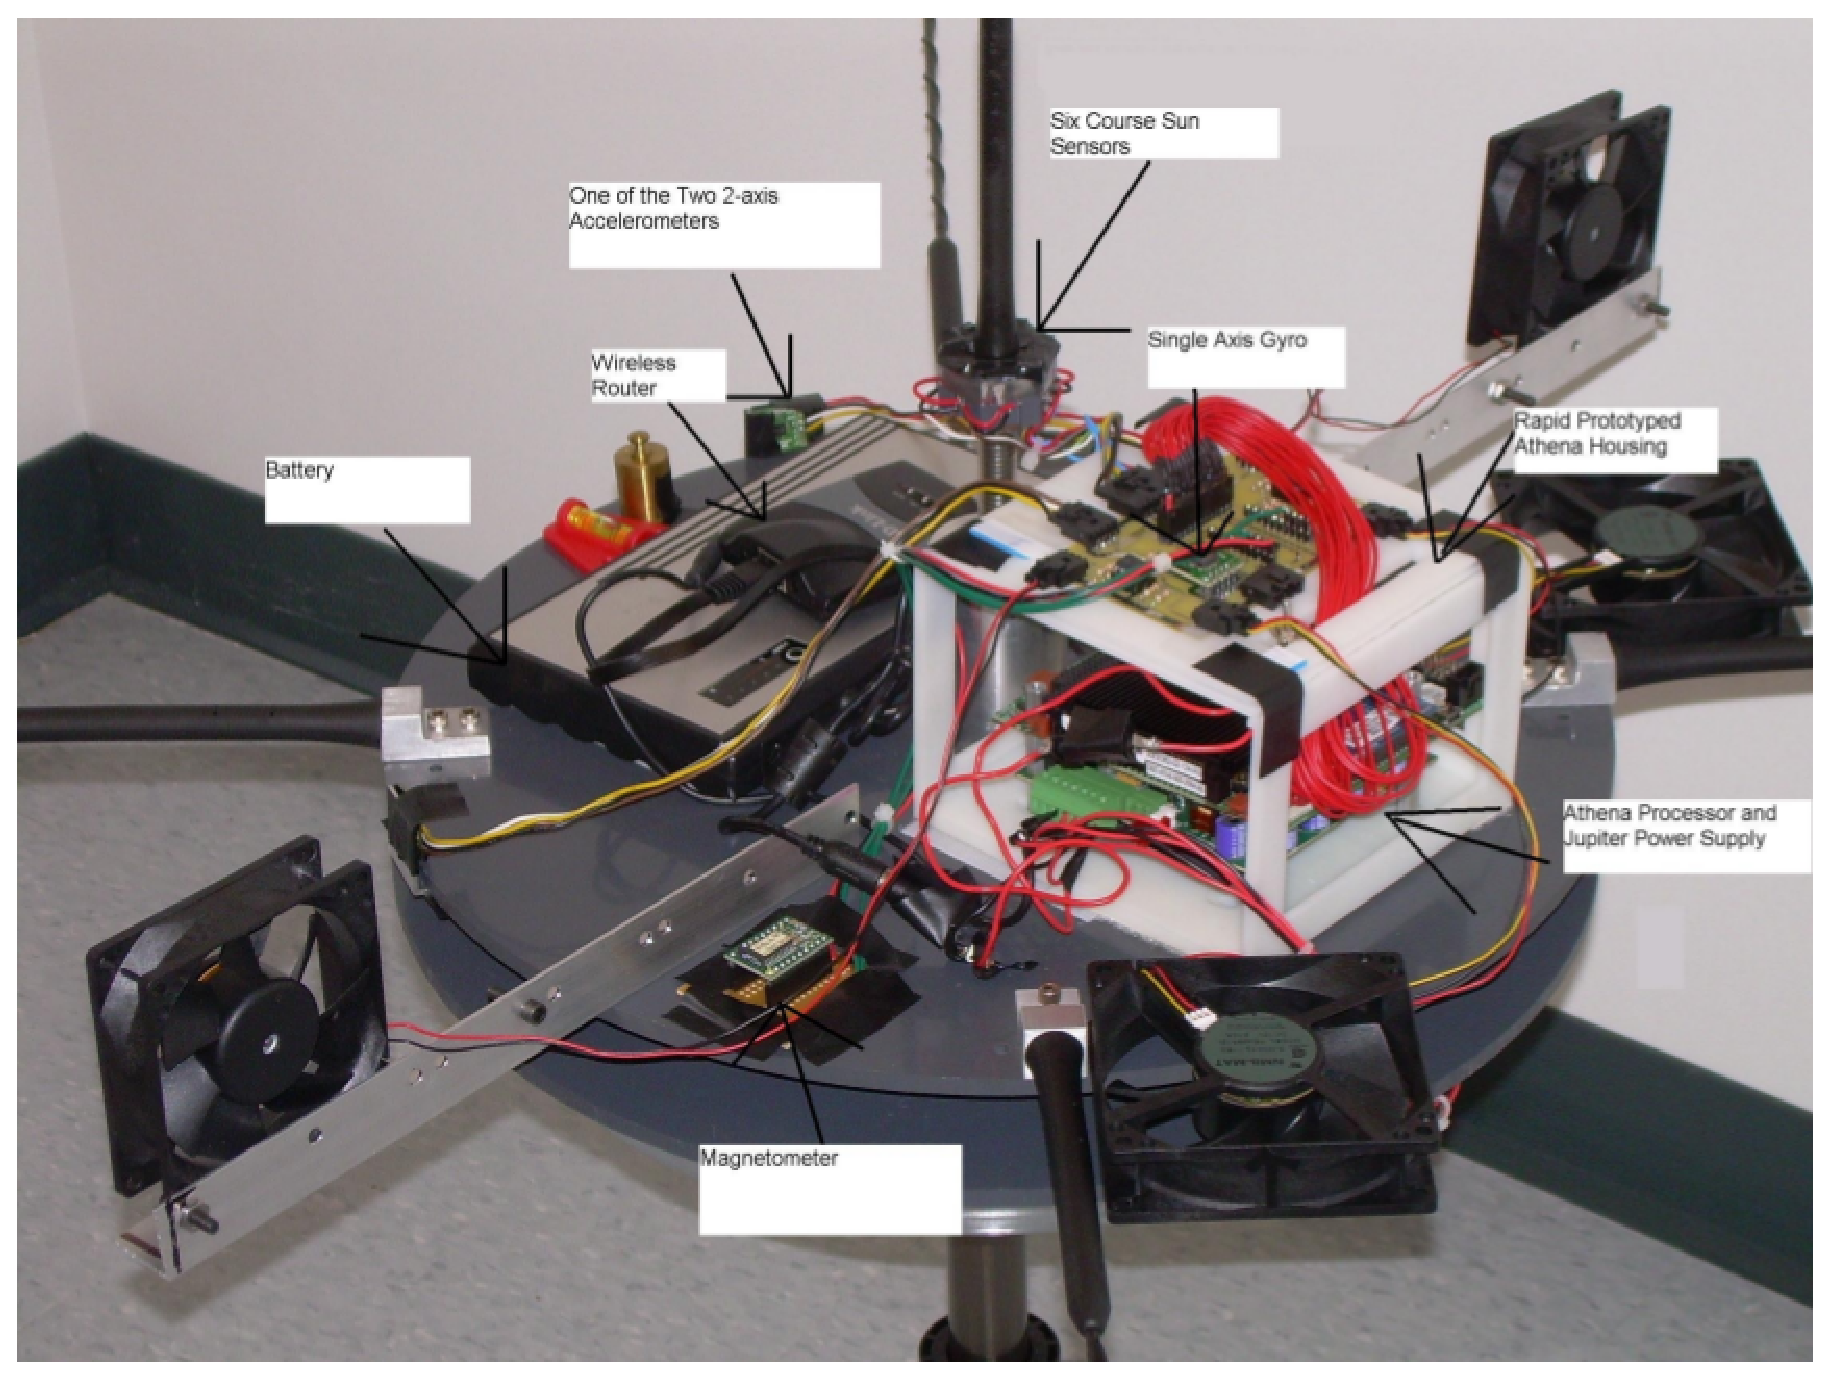
\psfig{file=figures/tsat_components.eps,height=4in}}
\caption{TableSat Components}
\label{fig:TSatComponents}
\end{figure}

\section{Flight Controller}
\label{sec:FlightController}

The onboard flight controller was an Athena PC from Diamond Systems powered by a Jupiter power supply and lithium-ion rechargeable battery.  The Athena processor and Jupiter power supply were mounted in a rapid prototyping housing with open sides for ventilation.  A custom printed circuit board designed by Jeff Kite \TODO{need footnote reference here?} was mounted on top of the rapid prototyping housing.  User Datagram Protocol (UDP) communication (Section \ref{sec:Messages}) to the base station is transmitted through a wireless access point.

\TODO{forgot cs student's name} created a C program based off of Vess' ``open-loop'' flight controller \cite{vessthesis} .  This program is responsible for listening to a UDP socket on the TableSat and performing a limited set of actions based on the message packets received from the base station.  The most common messages triggered actions like altering the voltages applied to the actuators, and scanning the sensor ports and sending the voltages back to the base station through UDP.

\section{Actuators}
\label{sec:Actuators}

In addition to the booms extending from the TableSat's deck, four single direction analog input computer fans were mounted to provide a source of thrust (Figure \ref{fig:TSatComponents}).  Two fans were mounted standing upright to provide radial torque.  One pointing clockwise and the other counter clockwise had their centers level with the pivot point inside the central hub and provided control of the rotation rate.  Two other fans were mounted facing down to provide limited opportunities for nutation control.

\section{Sensors}
\label{sec:Sensors}

Four classes of analog sensors were implemented in TableSat 1A's design; gyroscope (Section \ref{subsec:Gyroscope}), accelerometer (Section \ref{subsec:Accelerometer}), course sun sensor (Section \ref{subsec:CourseSunSensor}), and magnetometer (Section \ref{subsec:TripleAxisMagnetometer}).  These sensors and the four actuators filled all available analog ports on the onboard Athena flight computer.

\subsection{Gyroscope}
\label{subsec:Gyroscope}

Gyroscopes remain one of the most accurate sensors for detecting changes to a structure's angular body rates.  The issue with their use is that to increasing the accuracy of a gyroscope means using a heavier sensor.  Since any additional weight is a serious launch concern for a satellite, this research for NASA's MMS mission uses the gyro scope solely as a verification method.  The gyroscope selected for TableSat 1A is a single axis gyroscope that is mounted on the printed circuit board at the top of the flight controller housing.  The gyroscope is oriented to detect changes in body rates about the TableSat's z-axis although is mounted slightly above the center hub's pivot point so will pick up small signals from any limited nutation encountered.

\subsection{Accelerometer}
\label{subsec:Accelerometer}

Two 2-axis accelerometers are mounted at the circumference or TableSat's deck.  The sensors have a 2g resolution and are oriented such that one signal detects vertical acceleration and the other radial.  The rotational accelerometers ended up generating a distinguishable signal, but the vertical components of the accelerometers had such low signal to noise ratios that heavy filtering would be required to even attempt to detect the out of plane rotations.  Any significant nutations allowed by the limited 3-DOF design would damp out quickly enough to be eliminated before the filtering could identify the signal.  Given these severe limitations in the sensor's measurements, for the purpose of this thesis the accelerometer measurements are ignored.

\subsection{Course Sun Sensor}
\label{subsec:CourseSunSensor}

The course sun sensor for UNH TableSat 1A was constructed from a hexagonal piece of PVC pipe with a photodiode mounted in each face (Figure \ref{fig:CSS}).  Photodiodes are light detectors that convert captured light to electricity.  Given the inability to use the gyroscope and the accelerometer's high level of noise, the course sun sensor became the most reliable sensor.  Each photo diode detected light level in its field of view and would generate a voltage generally proportional to that value.  The photodiodes were mounted above the center hub and faced out around the spin plane.  By placing a single light source in a dark room, the course sun sensor's voltages could be used to calculate the angular displacement about the body's z-axis.


\begin{figure}[H]
\centerline{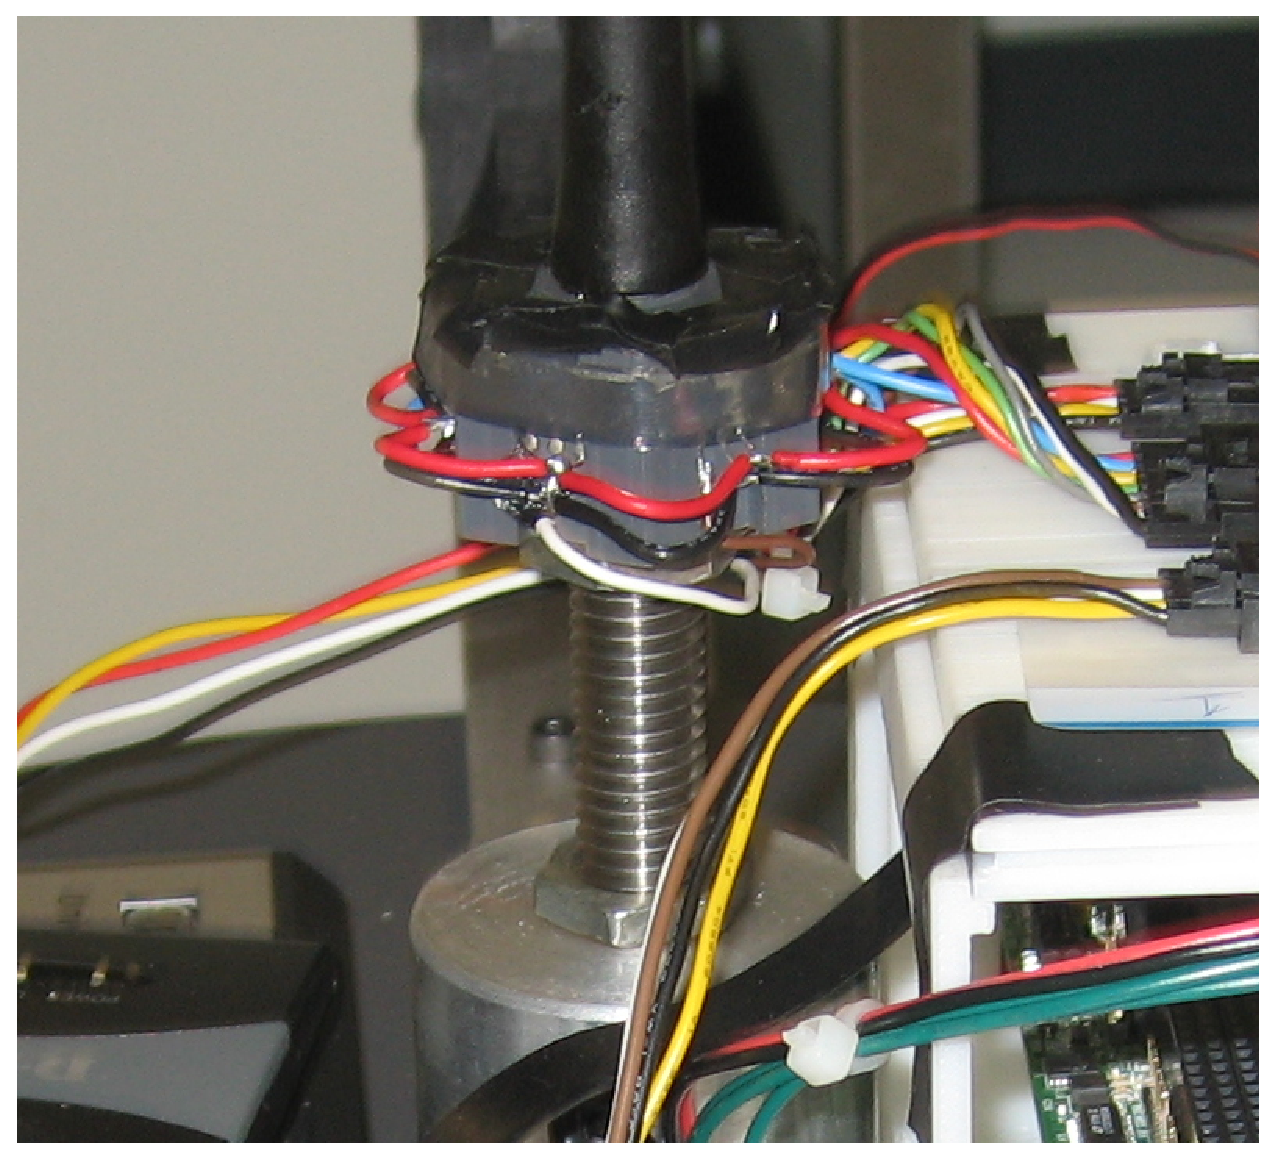
\psfig{file=figures/css.eps,height=2in}}
\caption{Course Sun Sensor Configuration}
\label{fig:CSS}
\end{figure}

Calculating the angular displacement about the body's z-axis is done using a method similar to a resultant force calculation.  Assuming all of the photodiodes volts per lumen rates are consistent, the voltages can be described as an equivalent force it the direction of the photodiode face.  Each force is decomposed into x and y components and then summed into a resultant force vector who's angle is used to represent the angular displacement of the TableSat.  Even though this method is fairly simplistic and that individual sensor voltage readings contained a moderate level of noise, this method proved to generate a very reliable and clean signal before even using filtering and estimation techniques.

\begin{subequations}
\begin{align}
V_{css\_x} & = \sum\limits_{i=1}^6 (V_{css\_x} - V_{css\_base}) \cos \left( \frac{2\pi}{6} (i-1)\right) \\
V_{css\_y} & = \sum\limits_{i=1}^6 (V_{css\_x} - V_{css\_base}) \sin \left( \frac{2\pi}{6} (i-1)\right) \\
\psi & = \tan^{-1} \frac{V_{css\_y}}{V_{css\_x}}
\end{align}
\end{subequations}

\begin{figure}[H]
\centerline{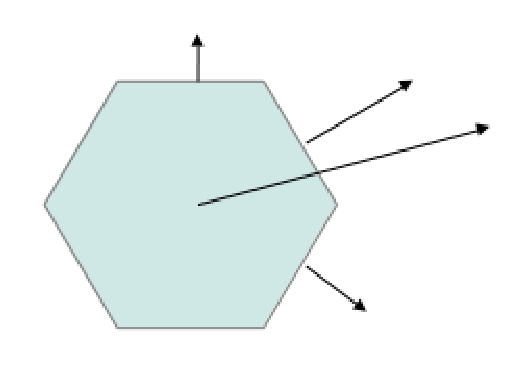
\psfig{file=figures/css_vectors.eps,height=1in}}
\caption{Photodiode Resultant Force Calculation for Yaw}
\label{fig:CSSVectors}
\end{figure}


\subsection{Triple Axis Magnetometer}
\label{subsec:TripleAxisMagnetometer}


\section{User Data Gram Protocol vs. Transmission Control Protocol}
\label{subsec:UDPTCP}

Communication between the controller and the experimental TableSat is
negotiated over a User Datagram Protocol (UDP) socket.  Both the
controller and TableSat read and write over port 9877.  UDP is used for
a stateless connection more generally used for pushing data over a
large number of connections.  The other common communication protocol
is Transmission Control Protocol (TCP) where a session is established
between server and client and successful transferral of data is
acknowledged by the recipient.

The advantage to using UDP for the UNH TableSat 1 is that the satellite
side code could be largely based off of Melissa Vess' work on her
TableSat thesis where the control loop was implemented on-board, and
the UDP connection was used to infrequently poll for data or modify
sensor calibration values.  The UDP connection has the slight advantage
of being able to transmit and receive packets without needing to wait for
acknowledgments.  This could save a small fraction of time, but on modern
hardware and with the small bandwidth usage this advantage is negligible.

Disadvantages to implementing the control interface through UDP include
the possibility of packet loss where the sender submits a packet, but
it gets corrupted or dropped.  Since UDP is a stateless connection, the
sender doesn't wait for an acknowledgment which in this case would not come.
This issue is handled by the communications module.  If the control loop rate
on both updating the actuator voltages and polling sensor data is fast enough,
a dropped packet would not matter much since a new updated set of values
would be soon to follow.  Issues could be caused if the completion of a
code loop was dependent on a packet coming in.  If dropped, the control
loop could block until the next packet is received.  This was one issue
encountered in the project version [sec:ControlLoopinSimulink].


\section{Messages}
\label{sec:Messages}


The packet structure used for this project is the same as used by Melissa Vess \TODO{add cite}.
Each UDP packet is comprised of a packet header and data payload.  The packet
header format remains constant for all messages containing five octets of data.

\begin{center}
    \begin{tabular}{| l | l |}
    \hline
    Header Octet & Description \\ \hline
    h1 & Message Number (0 to 255) \\ \hline
    h2 & Flags (0 - 255) \\ \hline
    h3 & Message Size (0 - 255) \\ \hline
    h4 & Message Size (0 - 255) \\ \hline
    h5 & 0 \\ \hline
    \end{tabular}
\end{center}

The first octet (h1) contains the message number that matches to a predefined list
of messages known by both the sender and recipient.  This is used to specify
how the data in the payload is to be used.

The second octet (h2) is reserved for flags.  For some messages, flags can be
set for additional data.  These are not used in the final implementation of
UNH TableSat 1A.

The third (h3) and fourth (h4) header octets define the size of the data's payload, so when reading
data in from a buffer, the header can inform the recipient how many bytes need
to get read in from the buffer in order to get to the end of the packet.  For
payloads less than 256 bytes only the fourth header byte is needed.  For
payloads larger than 255 bytes the following formula is used to specify the
message size headers.

\begin{align}
h4 &= mod(size, 256) \\
h3 &= floor(size / 256)
\end{align}

The only meta data provided along with the payload beyond the data's size is
an 8 bit message number.  Both UNH TableSat 1A and the control station have
identical message list definitions.

\begin{center}
    \begin{tabular}{| l | l | l | l |}
    \hline
    Message Id & Payload Size & Data Type & Message Description \\ \hline
    2 & 1 octet & unsigned int & Set run mode \\ \hline
    4 & 1 octet & unsigned int & Set run mode \\ \hline
    18 & 4 x (8 octets) & float & Set fan speed \\ \hline
    19 & 1 octet & unsigned int & Set log record mode \\ \hline
    20 & 1 octet & unsigned int & Request sensor reading \\ \hline
    22 & 1 octet & unsigned int & End of sensor log \\ \hline
    23 & 8 octets & float & Request sensor log data \\ \hline
    33 & 8 octets & float & Set log sample rate \\ \hline
    63 & 15 x (8 octets) & float & Sensor readings \\ \hline
    64 & 16 x (8 octets) & float & Sensor log entry \\ \hline
    65 & 8 octets & float & Sensor log size \\ \hline
    104 & 1 octet & unsigned int & Ack run mode \\ \hline
    118 & 1 octet & unsigned int & Ack fan volt \\ \hline
    119 & 1 octet & unsigned int & Ack sensor log run mode \\ \hline
    133 & 1 octet & unsigned int & Ack log sample rate \\ \hline
    \end{tabular}
\end{center}
